\documentclass[a4paper,12pt]{article}
\usepackage[toc,page]{appendix}
\usepackage{listings}
\usepackage{hyperref}
\usepackage{graphicx}
\usepackage[skip=0pt]{caption}
\usepackage{multicol}
\usepackage{float}
\usepackage[margin=1in]{geometry}

\begin{document}

\renewcommand{\thelstlisting}{\thesection-\arabic{lstlisting}}
\renewcommand{\thefigure}{\arabic{section}-\arabic{figure}}
\setlength{\floatsep}{0pt plus 2pt minus 2pt}
%\setlength{\intextsep}{0pt plus 2pt minus 2pt}
%\setlength{\textfloatsep}{0pt plus 2pt minus 2pt}

\title{Introduction to Digital Libraries Assignment \#1}
\date{February 11, 2015}
\author{James Tate II}
\maketitle

\section{Introduction}
This assignment required downloading \emph{tweets} from \emph{Twitter} using its API and processing the HTTP URIs
those tweets contained. The URIs were dereferenced from their original http://t.co/... form to their final
URI after following all redirects. The representation obtained by dereferencing the final URI was recorded
for later use. The URIs were also given an age by the CarbonDate utility. This report includes some statistical
data gathered along the way.

\section{Methodology}
The data for this assignment was obtained and processed in several stages rather than all at once. 
This enabled agile development, and also did not require much effort be put into usability or maintainability 
of the code used at each stage. Six significant Python scripts were developed, along with a library of
miscellaneous functions not worth mentioning. Three Bash scripts were also developed. Third-party resources
included CarbonDate, casperjs, phantomjs and CherryPy, along with the Python standard library, wget, curl and
numerous other GNU utilities.

\subsection{Downloading Tweets}
The first step was, of course, to download enough tweets that 10000 URIs were able to be analysed after culling
the unusable tweets. Tweets were downloaded using Twitter's streaming API. A list of 23 keywords\footnote{See
Appendix A for a list of the keywords used.} was used in
the \texttt{filter} endpoint on the streaming API, as special permission is required to use the \texttt{firehose}
endpoint. Because the streaming API was used, retireved tweets were newly published tweets at the time of
retrieval. The JSON of each tweet was saved to an output file for later processing. The command to download
tweets is shown in listing 2-1. The output file is always \texttt{output.log}.
\begin{lstlisting}[basicstyle=\ttfamily,caption={Downloading Tweets}]
    ./download_tweets.py
\end{lstlisting}

\subsection{Culling Tweets}
The first step in culling tweets was a na\"{\i}ve attempt to omit tweets with adult content. \texttt{grep}
was used as shown in listing 2-2 to remove tweets containing the string \texttt{porn} in any case,
regardless of position in a word.
\begin{lstlisting}[basicstyle=\ttfamily,caption={Removing Naughty Tweets}]
    grep -vi "porn" output.log > output.log.2
\end{lstlisting}
The next step in culling tweets was to actually remove tweets that did not contain any HTTP URIs. This was
accomplished as part of the next Python script's functionality. This script also extracts the HTTP URIs from
 the tweet, and saves them along with the tweet text each in their own file in a directory just for that
tweet. The directory name is the ID of the tweet. All these tweet directories are in one directory with
no other items. A sample directory tree of a tweet with two URIs is show in
listing 2-3. The command to extract tweets, skipping tweets without URIs, is shown in listing 2-4.
\begin{lstlisting}[basicstyle=\ttfamily,caption={Tweet Directory Structure}]
    tweets/
        560614568091602944/
            text
            url.0
            url.1
\end{lstlisting}
\begin{lstlisting}[basicstyle=\ttfamily,caption={Extracting Tweets}]
    ./extract_tweets output.logs.2
\end{lstlisting}

\subsection{Dereferencing URIs}
Before the URIs can be analysed, they need to be dereferenced using curl to obtain their final URIs. While
obtaining
the final URIs, I went ahead and retrieved the representation of the resource by dereferencing each URI in
wget. The final URI is the last URI obtained by dereferencing each URI with an HTTP \texttt{HEAD} command,
and following the chain of redirects. Anytime a URI response is a redirect (HTTP status 3XX), the \texttt{Location} header
in the response contained the next URI to be dereferenced.\cite{rfc2616} Eventually, each URI would be
dereferenced into a successful (2XX), client error (4XX) or server error (5XX) response.\footnote{Actually,
if the URI chain hit 51 URIs due to encountering 50 redirects, it would stop because curl would throw an
exception and quit. This did not happen in my sample, however.} The command to dereference the URIs is shown
in listing 2-5.
\begin{lstlisting}[basicstyle=\ttfamily,caption={Dereferencing URIs}]
    ./dereference_URIs.py
\end{lstlisting}
This script uses the Python \texttt{subprocess.Popen} function to call curl and wget without blocking the
Python thread. Up to 128 combined curl and wget processes were allowed to run simultaneously, which
allowed over 10000 URIs to be dereferenced by both curl and wget in about 20 minutes. The curl and wget
commands reside in their own Bash scripts which contain a little boilerplate for managing the output.
However, the actual curl and wget commands used are shown in listings 2-6 and 2-7, respectively.
\begin{lstlisting}[basicstyle=\ttfamily,caption={Curl Command}]
    curl -I -L -m 60 "$url" > "tweets/$1/headers.$index" 2>&1
\end{lstlisting}
\begin{lstlisting}[basicstyle=\ttfamily,caption={Wget Command}]
    wget -t 2 -T 30 -E -e robots=off --trust-server-names -U \
        `Mozilla/5.0 (X11; U; Linux i686; en-US; rv:1.8.1.6) '\
        `Gecko/20070802 SeaMonkey/1.1.4' -P "$dir/" "$url" \
        > "$dir/wget.output" 2>&1
\end{lstlisting}
The curl command doesn't have too much going on. The flags tell it to make HEAD requests instead of GET
requests, follow all redirects and use a maximum timeout of 60 seconds. The argument is the URI to be
dereferenced. The output is redirected to the headers file for this URI in this tweet's directory,
and stderr is also redirected to that file.

The wget command, on the other hand, is very busy. The flags, in this order, set maximum number of tries
to two, set the timeout for all types of network operations to 30 seconds, ensure file extensions are set to
correct values even if the URI does not have the correct extension, turn off \texttt{robots.txt} processing,
sets the output filename to filename of the last URI (after redirection), sets the user-agent to a
non-robot user-agent and sets the output directory to the content directory for this URI. The argument is
the URI to be dereferenced and stdout and stderr are redirected to a log file in the content directory.

The representation is stored in a separate subfolder of the tweet directory from the other information.
The final directory structure looks like the sample shown in listing 2-8.
\begin{lstlisting}[basicstyle=\ttfamily,caption={Sample Final Directory Structure}]
    tweets/
        560614568091602944/
            text
            url.0
            url.1
            headers.0
            headers.1
            content.0/
                wget.output
                filename_from_URI.html
            content.1/
                wget.output
                different_filename.htm
\end{lstlisting}
The \texttt{dereference\_URIs.py} script saves some statistics about what it did in the
\texttt{download.stats} file. The statistics include the IDs of any tweets for which there were errors
when running curl or wget. These tweets (and all their URIs) will be removed in the next step.

\subsection{Combining Data}
After the URIs are dereferenced, the data is not yet in an easily accessible and modifiable form. With
multiple flat files in multiple directories, data access is slow and error-prone. This step combines the
data we care about into one large array, which is stored in a single file in JSON. The data we care about
(and have so far) is the tweet ID, tweet text, initial URIs, final URIs, tweet creation time
and HTTP status codes. The \texttt{summary.py} script gathers all this disparate information together.
It also removes the tweets with URIs that generated errors in curl or wget from the disk and the summary.
I ran these two functions separately,
but they could be run together if all the command-line options are combined. See listing 2-9 for the two
commands used to generate the summary and remove tweets with errors. Also in listing 2-9 is the
\texttt{mv} command used to put the summary back after it was rewritten.
\begin{lstlisting}[basicstyle=\ttfamily,caption={Summarization and Errored Tweet Removal}]
    ./summary.py -l tweets -p -t output.log.2 \
        > tweets.summary.json
    ./summary.py -r tweets.summary.json \
        -d download.stats -x -p \
        > tweets.summary.json.temp
    mv tweets.summary.json.temp tweets.summary.json
\end{lstlisting}
The first command loads tweet data from the \texttt{tweets} directory, prints the summarization JSON
to stdout, and uses the tweet JSON output from a few steps ago to add one piece of metadata not found
in a flat file: the creation time of the tweet. The second command reads the summarization generated
by the previous command, excludes tweets that had derference errors, and deletes those tweets from
the disk. The output is printed to a temporary file, which is then moved back to its original
filename. At this point, we have all the data we need except the age of the URIs.

\subsection{Getting URI Age}
To get the URI age, the CarbonDate utility is used. This utility, created at ODU, checks web archives,
Google, Topsy, Bitly and the \texttt{Last-Modified} header to hopefully find the earliest date that
each URI was seen on the web. The earliest found date/time among the results from these services is
subtracted from the creation time of the tweet containing the URI to determine how old the URI was
when it was posted on Twitter. For some URIs, none of these services returned a date/time, so we can
only assume that the creation date of the tweet containing the URI is also the birthday of the URI.
The calculated age is stored in the summary JSON for later processing by the command in listing 2-10.
\begin{lstlisting}[basicstyle=\ttfamily,caption={Getting the URI Age}]
    ./carbondate_URIs.py tweets.summary.json \
        > tweets.summary.with_delta.json
    mv tweets.summary.with_delta.json \
        tweets.summary.json
\end{lstlisting}
The \texttt{mv} command returns the output summary with URI ages to its original filename.

\subsection{Getting Statistics}
Now that all data has been retrieved and calculated, we can generate some statistics. The
\texttt{summary.py} script is used again, with a new option, to get the statistics. This is shown in
listing 2-11.
\begin{lstlisting}[basicstyle=\ttfamily,caption={Generating Statistics}]
    ./summary.py -r tweets.summary.with_delta.json -S
\end{lstlisting}
This command reads the summary JSON and prints the statistics for the first 10000 URIs listed in
that file. The statistics calculated will be described in Section 3. If the \texttt{-s} option was
used instead, the statistics would be calculated for every URI in the summary file.


\section{Statistics}
I had to download over 35000 tweets to get 10000 usable URIs after all the various reasons for
excluding a tweet or URI. About half the tweets did not include URIs, and a third of the remaining ones
only included media URIs --- links to Youtube or directly to images. Media URIs were not included in
this study. Of the remaining tweets, one or more of the URIs in a few hundred of the tweets failed to
be dereferenced in either curl or wget, so the entire tweet was excluded.

\subsection{HTTP Status Codes}
Each URI not removed from the sample had at least two HTTP status codes. The first was always a 301
returned when dereferencing the initial http://t.co/... URI. There were 9711 redirect codes beyond
those initial 10000 in the sample data. About 93\% of the URIs eventually resolved to a 200 status
which indicates a webpage was successfully retrieved. About 6.5\% had client errors such as a 404,
and only 15 URIs, 0.15\%, ended with a server error.

The histogram in Figure 3-1 illustrates the
distribution of HTTP status codes received in the four common ranges (success, redirect, client error
and server error). The histogram in Figure 3-2 shows the frequency of the number of redirects
required to dereference a URI until a non-redirect status is returned.
\begin{figure}[H]
    \centering
    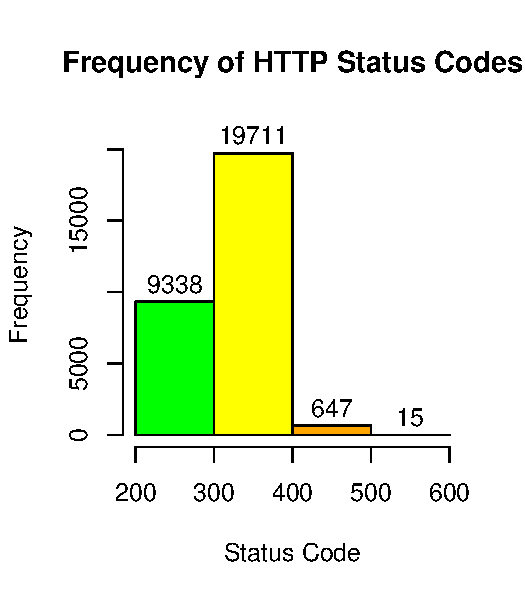
\includegraphics{stats/http_status_codes.pdf}
    \caption{Frequency of HTTP status codes in histogram by sequential category.}
\end{figure}
\begin{figure}[H]
    \centering
    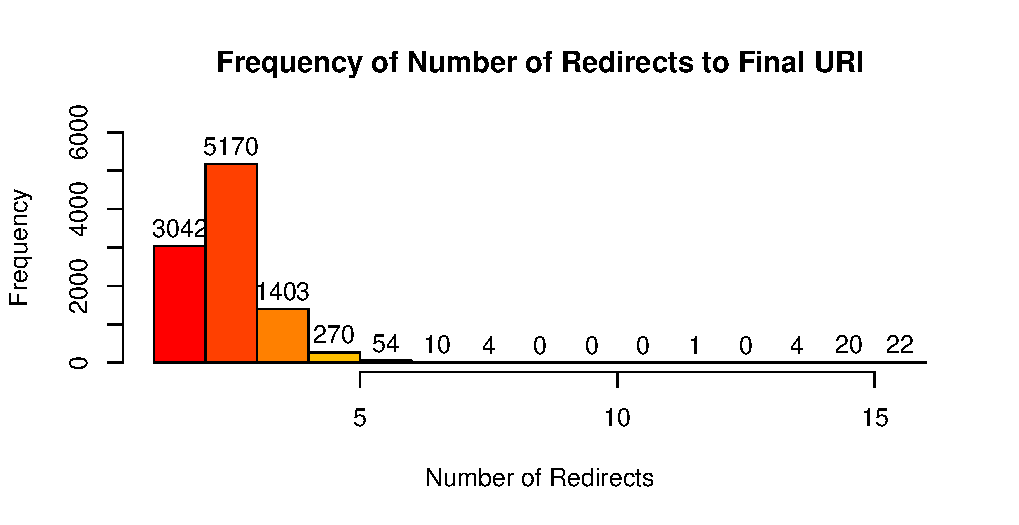
\includegraphics{stats/num_redirects.pdf}
    \caption{Frequency of number of redirects required to fully dereference a URI.}
\end{figure}

\subsection{Unique and Duplicate URIs}
One of the fundamental features of Twitter is the ability to \emph{retweet} another user's tweet.
If the original tweet included a URI and my filter caught it, a retweet during the time I was
downloading tweets would have probably been downloaded also. Users also quite frequently share the
same link without retweeting, but just by pasting the same link into the tweet text. Both of these
situations result in duplicate URIs.

In my sample set, there were 7376 unique http://t.co/... URIs,
but only 5375 unique final URIs. This means there were 2001 URIs that were duplicates not from
retweets, but from users pasting the same URI independent of each other.  
Inversely, the number of repeated http://t.co/... URIs was 776 while the number of repeated final
URIs was 1151. Figure 3-3 is a bar graph of the number of unique and repeated URIs. 
\begin{figure}[H]
    \centering
    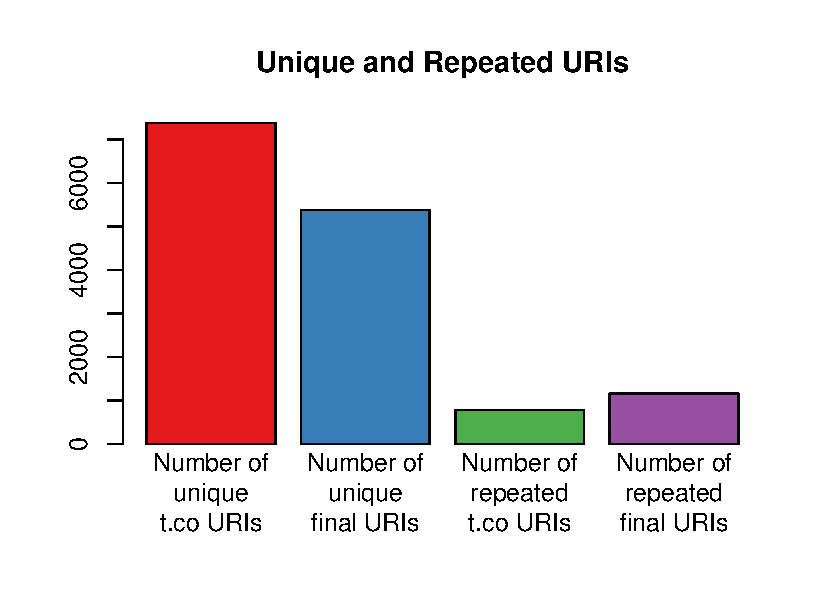
\includegraphics{stats/unique_and_dupe.pdf}
    \caption{Bar chart showing the number of unique and repeated initial and final URIs.}
\end{figure}

\subsection{Quantity of URIs per Tweet}
\begin{figure}[H]
    \centering
    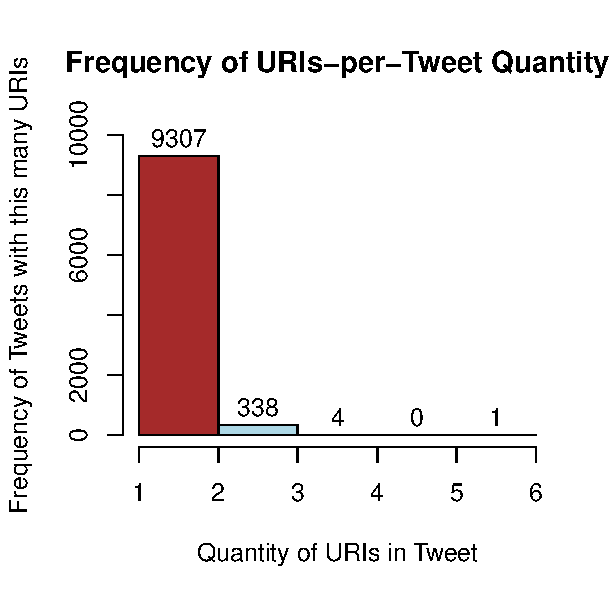
\includegraphics{stats/uris_per_tweet.pdf}
    \caption{Frequency of HTTP status codes in histogram by sequential category.}
\end{figure}
Figure 3-4 shows the frequency of tweets with a given number of URIs in the sample data. The
histogram clearly shows that the vast majority of tweets only contain one URI.

Figures 3-5 and 3-6 are histograms showing the frequency of URI multiplicity in my sample set.
For these two figures, outliers, specifically multiplicites above 15, have been removed from the
graph for a more appealling image. These outliers are less than 1\% of the sample data. The most
striking sample from those outliers is one final URI that was present in 170 tweets, all of which
were retweets. This means the same initial URI is present in the sample set 170 times as well.
\begin{figure}[H]
    \centering
    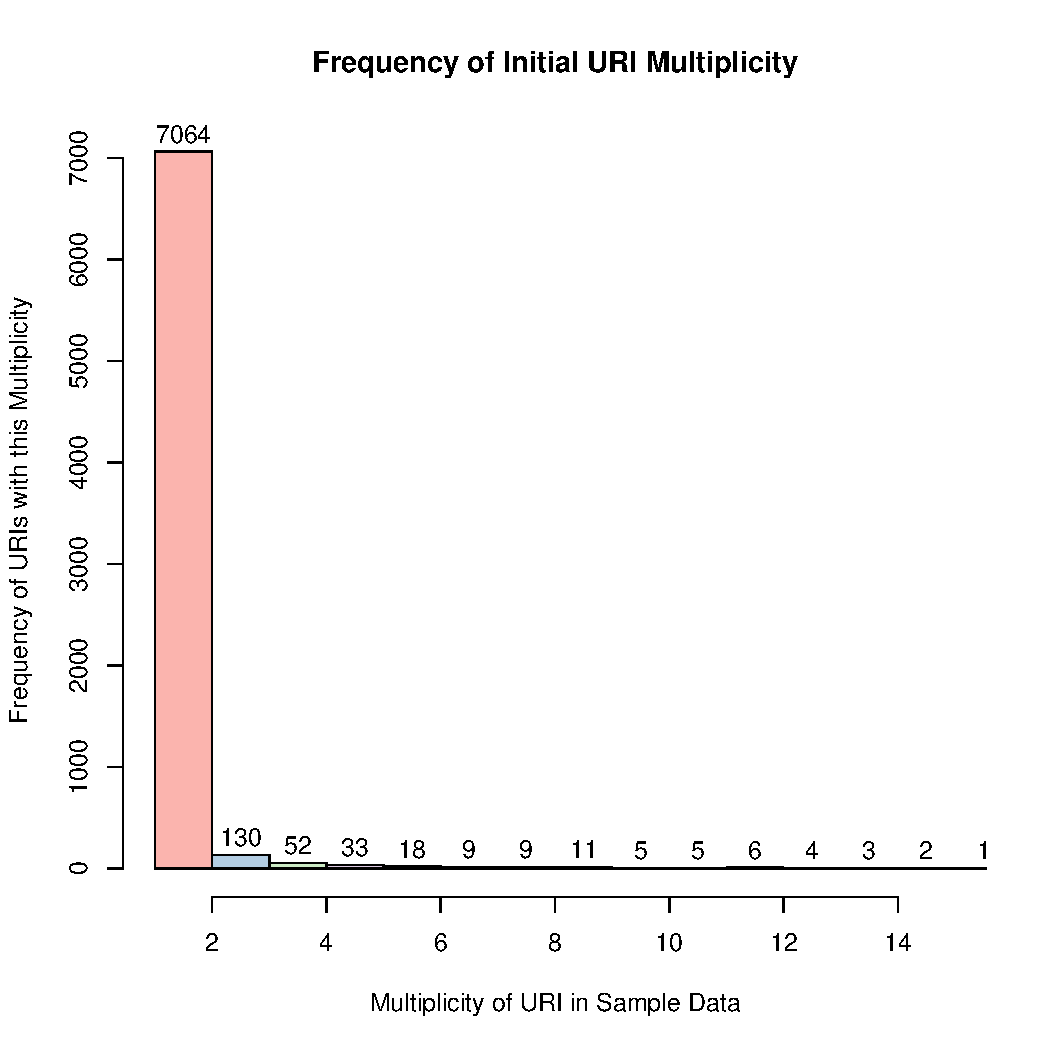
\includegraphics{stats/frequency_initial_uri_multiplicity.pdf}
    \caption{Histogram showing frequency of initial URI multiplicity, with outliers excluded.}
\end{figure}
\begin{figure}[H]
    \centering
    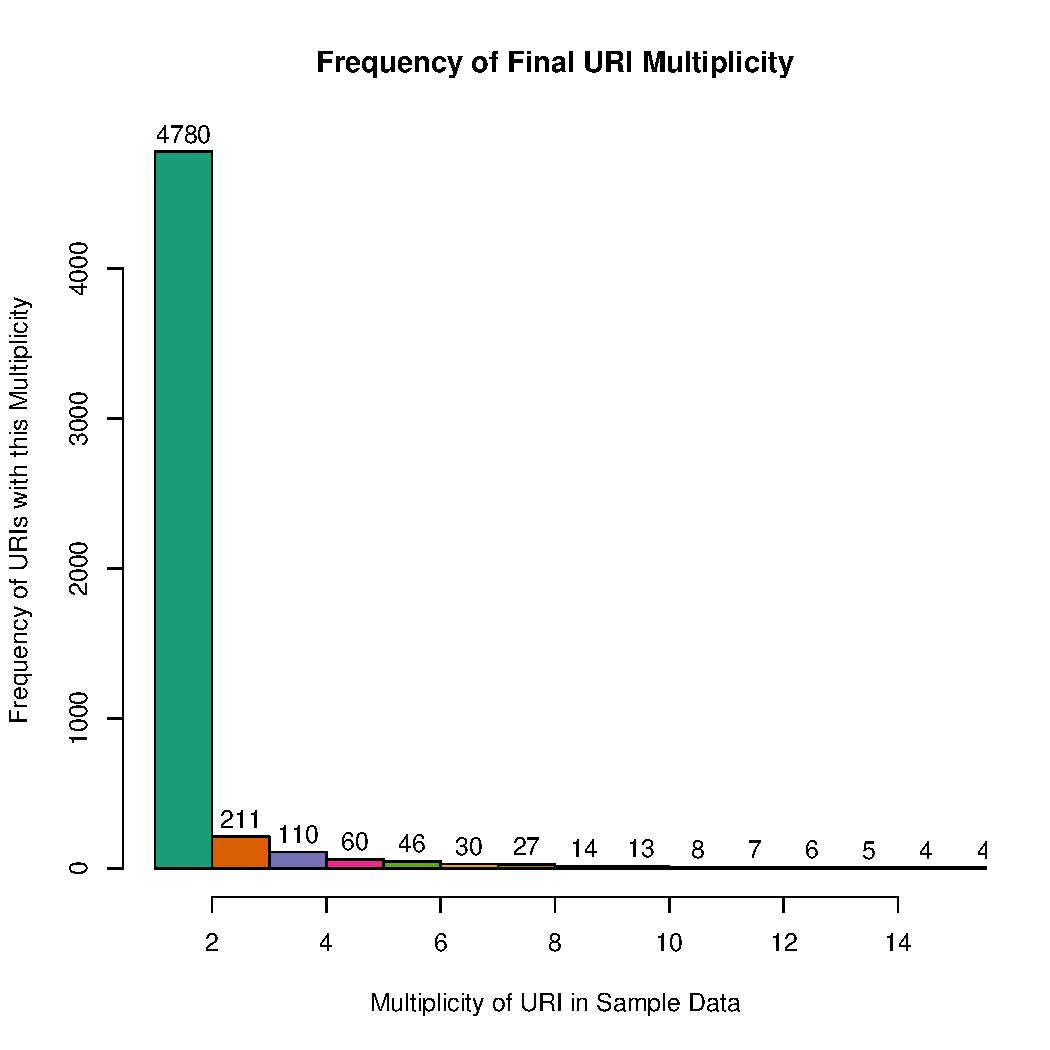
\includegraphics{stats/frequency_final_uri_multiplicity.pdf}
    \caption{Histogram showing frequency of final URI multiplicity, with outliers excluded.}
\end{figure}

\subsection{Age of URIs}
As previously described, the age of the URIs was determined by subtracting the CarbonDate
``birthday'' of the URI from the tweet creation date and time. The difference was zero if
CarbonDate was not able to find any source for the URIs birthday or if the source was the
tweet from which the URI was retrieved. From these ages, I calculated some statistical values:
\begin{itemize}
    \item Median Age: 79.9 days
    \item Mean Age: 29.6 minutes
    \item Standard Deviation: 282 days
    \item Standard Error: 2.81 days
\end{itemize}
Of the 10000 URIs, 4231 were determined to have an age of zero, meaning the earliest known
reference was the tweet from which they were retrieved. The oldest URI was 11.2 years old.
This URI\footnote{\url{http://www.ewtn.com/library/HOMELIBR/FOSSILR.TXT}} appears to be a
scholarly article about the fossil record, but is from a dubious source. Figure 3-7 is a
histogram of the ages of the URIs in the sample set.
\begin{figure}[H]
    \centering
    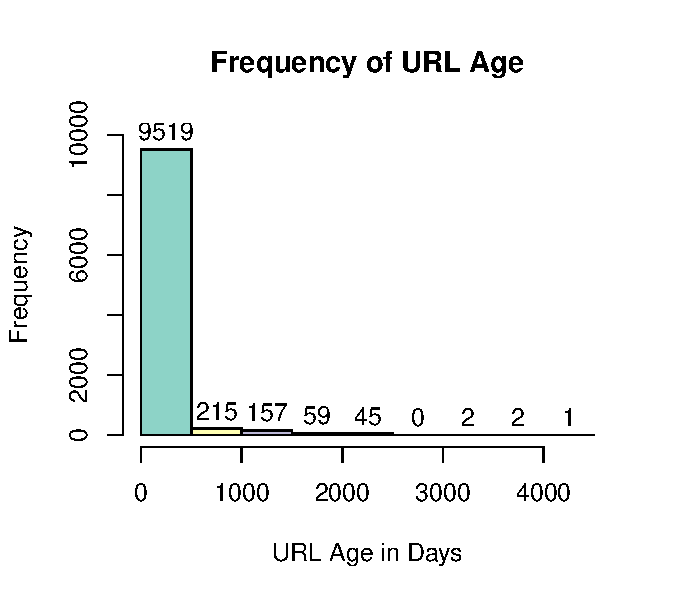
\includegraphics{stats/time_deltas.pdf}
    \caption{This histogram illustrates the frequency of URI age, as determined by CarbonDate.}
\end{figure}



\clearpage
\begin{appendices}

\section{Streaming API Filter Keywords}
These keywords were selected arbitrarily. Keywords were added to the list until the streaming
API seemed to pull tweets at a strong, consistent rate.
\begin{multicols}{3}
\begin{itemize}
    \item python
    \item fsf
    \item foss
    \item coding
    \item programming
    \item fedora
    \item rhel
    \item dovetail
    \item woodworking
    \item blizzard
    \item snowstorm
    \item colorado
    \item virginia
    \item internet
    \item library
    \item libraries
    \item json
    \item lemonade
    \item woodchuck
    \item iasip
    \item league
    \item awesomenaut
    \item tf2
\end{itemize}
\end{multicols}

\end{appendices}




\begin{thebibliography}{9}
\bibitem{rfc2616}
    R. Fielding, et. al.,
    \emph{Hypertext Transfer Protocol -- HTTP/1.1}.
    \url{https://www.ietf.org/rfc/rfc2616.txt}
    June 1999.


\end{thebibliography}

\end{document}
